%\documentclass[10pt]{llncs}


%\usepackage{amsmath}
%\usepackage{graphicx}
%\usepackage{subfigure}

%\usepackage{alltt}
%\usepackage{placeins}

%\usepackage{fancyvrb}


   \DefineVerbatimEnvironment
     {code}{Verbatim}
     {fontsize=\small,samepage=true}
% ,xleftmargin=0.6cm
%\begin{document}


%\title{Obsidian:\\A Domain Specific Embedded Language\\for Parallel Programming of Graphics Processors}
       

%\author{Joel Svensson \and Mary Sheeran \and Koen Claessen}
%\institute{Chalmers University of Technology, G\"oteborg, Sweden}

%\date{}
%\maketitle

\subsection*{Abstract}

We present a domain specific language, embedded in Haskell, for general
purpose parallel programming on GPUs. Our intention is to explore the use of
{\em connection patterns} in parallel programming. We briefly present our
earlier work on hardware generation, and outline the current state of GPU
architectures and programming models. Finally, we present the current status
of the {\em Obsidian} project, which aims to make GPU programming easier,
without relinquishing detailed control of GPU resources. Both a programming
example and some details of the implementation are presented. This is a
report on work in progress.

%\end{abstract}


\subsection{Introduction} 

%% table 


\begin{figure}
\begin{center}
  \begin{tabular}{  l | r | r}
    %\hline
    Kernel               & Threads   & ms / grid   \\ \hline
    bitonic\_sort(CUDA)  & 512       & 30.28       \\      
    tsort1               & 512       & 15.82       \\
    tsort2               & 256       & 11.64       \\ 
    vsort1               & 512       & 14.96       \\ 
    vsort                & 256       &  9.33       \\ 
    %\hline
  \end{tabular}
\end{center}
\label{fig:table}
\caption{Table is showing the time it takes for a grid of 32678 blocks of 
threads to execute.Each grid was launched 1000 times, the total execution time 
was then divided by 1000 to get the listed figures. The GPU used is a NVIDIA GTX480} 
\end{figure}


%----------------------------------------------------------------------------

Graphics Processing Units (GPUs) are parallel computers with hundreds 
to thousands of processing elements. The CUDA and OpenCL languages  
make available the power of the GPU to programmers interested in general 
purpose computations. In CUDA and OpenCL, the programmer writes {\em kernels}, 
Single Program Multiple Data (SPMD) programs that are executed by groups 
of threads on the available processing elements of the GPU.  

CUDA and OpenCL are general purpose programming languages, mirroring the 
increased capabilities of a modern GPU to target that domain. However, these 
languages lack compositionality. 
Also, being based in C/C++ means that the core idea in a program may
not be easily visible.  

\subsubsection{Embedded DSLs for GPGPU programming} 
We are aiming for a GPU programming language that is more
concise than mainstream
languages such as CUDA and OpenCL. 
Obsidian is a
domain specific embedded language (DSEL) implemented in Haskell.
When an Obsidian program is run, a representation of the program is created 
as a syntax tree. For more information on EDSL implementation see~\cite{COMPILEEDSL}.
The program representation generated when running an Obsidian program 
is compiled into CUDA code. We are also working on an OpenCL backend.

Our approach is different from that of other Haskell DSELs targetting
GPUs~\cite{ACCELERATE,NIKOLA,BARRACUDA}. 
We do not try to abstract away from 
all the peculiarities of GPU programming, but rather provide a higher 
level language in which to experiment with them.
For instance,
Accelerate provides a standard set of basic operations such as 
{\tt map}, {\tt reduce} and {\tt zipWith} as built in skeletons, implemented
with the help of small, predefined, hand-tuned CUDA kernels~\cite{ACCELERATE}. 
Obsidian, on the other hand, allows the user to experiment with the
{\em generation} of small kernels for fixed size array inputs
from higher level descriptions.
It is intended to allow the user to play with the kinds of tradeoffs that are important
when writing such high performance building blocks; in this paper, the main consideration
is the number of array elements of the input and output that are manipulated
by a single thread in the generated CUDA code.
An important aspect of Obsidian is the symbolic array representation used, along
with its associated {\tt sync} operation. As we shall see, the {\tt sync} operation
allows the programmer to guide code generation and control parallelism and thread
use~\cite{JSLIC}.




%Today there are number of EDSLs written in Haskell targeting 
%GPUs~\cite{ACCELERATE,NIKOLA,BARRACUDA}. We justify our work on yet 
%another by having a slightly different approach. We do not try to abstract away from 
%all the peculiarities of GPU programming but rather giving a higher 
%level language in which to experiment with them.
%trying to appeal to a slightly different target audience. 
%We try to cater not for the advanced functional programmer who wants to 
%run his programs on GPUs, but rather to offer a higher level 
%language to the CUDA/OpenCL hacker. 
%In this language we want the user to be 
%able to quickly experiment with the kind of tradeoffs that are important 
%when writing a high performance GPU kernel.

%Unlike the other approaches that are complementary to our Haskell GPU EDSL, 
%Obsidian does not provide the usual set of basic operations such as 
%{\tt Map}, {\tt Reduce} and {\tt ZipWith} as built in skeletons. We 
%want a language where the programmer can experiment with implementing 
%his or her own versions of these basic operations. So far, we make
%this possible in Obsidian through a {\tt Sync} operation and the Array 
%representation we use. The {\tt Sync} operation, using target domain 
%nomenclature, is the programmers tool to guide code generation and 
%obtain parallelism. The presentation of Obsidian here will be somewhat 
%cursory, for a more complete view of the various versions and approaches 
%we have tried, see~\cite{JSLIC}.
%More details on this later.

In Obsidian, a kernel that sums an array can be expressed as: 
\begin{codesize}
\begin{verbatim}
sum :: Array IntE -> Kernel (Array IntE) 
sum arr | len arr == 1 = return arr
        | otherwise    = (pure (fmap (uncurry (+)) . pair) 
                          ->- sync 
                          ->- sum) arr                       
\end{verbatim}
\end{codesize}
The result of running this kernel on an eight element input array, 
{\tt runKernel sum (namedArray ``input'' 8)}, is an intermediate representation 
of the computation (shown in slightly pretty-printed form): 
\begin{codesize}
\begin{verbatim}
arr0 = malloc(16)
par i 4 {
arr0[i] = ( +  input[( *  i 2 )] input[( +  ( *  i 2 ) 1 )] );
}Sync
arr1 = malloc(8)
par i 2 {
arr1[i] = ( +  arr0[( *  i 2 )] arr0[( +  ( *  i 2 ) 1 )] );
}Sync
arr2 = malloc(4)
par i 1 {
arr2[i] = ( +  arr1[( *  i 2 )] arr1[( +  ( *  i 2 ) 1 )] );
}Sync
\end{verbatim}
\end{codesize}
The named intermediate arrays in this representation are then laid 
out in GPU shared memory and CUDA code can be generated (here for arrays of length eight)\footnote{An alignment qualifier for shared memory 
has been omitted to save space in the listings showing generated code}: 
%\pagebreak
\begin{codesize}
\begin{verbatim}
__global__ void sum(int *input0,int *result0){
  unsigned int tid = threadIdx.x;
  unsigned int bid = blockIdx.x;
  extern __shared__ unsigned char sbase[];
  (( int *)sbase)[tid] = 
    (input0[((bid*8)+(tid*2))]+
     input0[((bid*8)+((tid*2)+1))]);
  __syncthreads();
  if (tid<2){
    (( int *)(sbase + 16))[tid] = 
      ((( int *)sbase)[(tid*2)]+
       (( int *)sbase)[((tid*2)+1)]);
  }
  __syncthreads();
  if (tid<1){
    (( int *)sbase)[tid] = 
      ((( int *)(sbase+16))[(tid*2)]+
       (( int *)(sbase+16))[((tid*2)+1)]);
  }
  __syncthreads();
  if (tid<1){
    result0[(bid+tid)] = (( int *)sbase)[tid];
  }
}
\end{verbatim}
\end{codesize}
%The CUDA code above is generated by issuing the command:
%\begin{codesize}
%\begin{verbatim}
%genKernel ``sum'' sum (namedArray undefined 8 :: Array IntE)
%\end{verbatim}
%\end{codesize}
%\noindent
%and the kernel code is generated for arrays of length eight.  



%----------------------------------------------------------------------------
\subsubsection{Arrays in Obsidian}

An array is represented by an indexing function and a length:
\begin{codesize} 
\begin{verbatim}
data Array a = Array (UWordE -> a) Word32 
\end{verbatim}
\end{codesize}
This array representation has served us well. It has these properties:
\begin{itemize} 
\item Fusion of operations is automatic.
\item It naturally describes a data-parallel computation suitable for CUDA/OpenCL generation.
\item Many basic operations can be implemented: {\tt map}, {\tt zipWith} etc.
\end{itemize}
Using this array representation in a DSEL is not new; the first occurence that we know of is in
Pan~\cite{PAN}. Similar array representations have also later been 
used in Feldspar~\cite{FELDSPAR}, and more recently also in the Repa library~\cite{REPA}.
Functions for indexing and getting the length of arrays are as follows:
\begin{codesize} 
\begin{verbatim}
(!) :: Array a -> UWordE -> a 
(Array ixf _) ! ix = ixf ix 

len :: Array a -> Word32
len (Array _ n) = n 
\end{verbatim}
\end{codesize}
%Implementing a {\em Functor} instance for the {\tt Array} datatype is possible:
A {\em Functor} instance for the {\tt Array} datatype is
\begin{codesize} 
\begin{verbatim}
instance Functor Array where 
  fmap f arr = Array (\ix -> f (arr ! ix)) (len arr) 
\end{verbatim}
\end{codesize}
Now, composed applications of {\tt fmap} will be automatically fused. This is 
illustrated in the example program below and the CUDA generated
from it.  
\begin{codesize} 
\begin{verbatim}
mapFusion :: Array IntE -> Kernel (Array IntE) 
mapFusion = pure (fmap (+1) . fmap (*2)) 
\end{verbatim}
\end{codesize}

\begin{codesize} 
\begin{verbatim}
__global__ void mapFusion(int *input0,int *result0){
  unsigned int tid = threadIdx.x;
  unsigned int bid = blockIdx.x;
  
  result0[((bid*32)+tid)] = ((input0[((bid*32)+tid)]*2)+1);
}
\end{verbatim}
\end{codesize}
Both of these code listings need explanation. In the Haskell 
code, {\tt mapFusion} has type {\tt Array IntE -> Kernel (Array IntE)};
{\tt Kernel} is a state monad that accumulates CUDA code as well as provides 
new names for intermediate arrays. Neither of these features of the monad 
is activated by this example though. The {\tt pure} function is defined 
using the monad's {\tt return} as {\tt pure f a = return (f a)}. In this case, 
it lifts a function of type {\tt Array IntE -> Array IntE} into 
a kernel. 

The generated CUDA code computes the result array using a number of threads 
equal to the length of that array. In this case, the kernel was generated
to deal with arrays of length $32$. The important detail to notice in the 
CUDA code is that there is no intermediate array created between the 
{\tt (*2)} and the {\tt (+1)} operations. 

The {\tt mapFusion} example could just as well have been implemented using 
the kernel sequential composition combinator, {\tt ->-}. 
\begin{codesize} 
\begin{verbatim}
mapFusion :: Array IntE -> Kernel (Array IntE) 
mapFusion = pure (fmap (*2)) ->- pure (fmap (+1)) 
\end{verbatim}
\end{codesize}
Exactly the same CUDA code is then generated.

In some cases, it is necessary to force computation of 
intermediate arrays. This can be used to share partial computations between 
threads and to expose parallelism. In Obsidian, the tool for this
is called {\tt sync}, a built-in kernel. Using {\tt sync} as follows prevents fusion of the
two operations:
\begin{codesize} 
\begin{verbatim}
mapUnFused :: Array IntE -> Kernel (Array IntE) 
mapUnFused = pure (fmap (*2)) ->- sync ->- pure (fmap (+1))
\end{verbatim}
\end{codesize}
The generated CUDA code now stores an intermediate result in local shared
memory before moving on. 
\begin{codesize} 
\begin{verbatim}
__global__ void mapUnFused(int *input0,int *result0){
  unsigned int tid = threadIdx.x;
  unsigned int bid = blockIdx.x;
  extern __shared__ unsigned char sbase[];
  (( int *)sbase)[tid] = (input0[((bid*32)+tid)]*2);
  __syncthreads();
  result0[((bid*32)+tid)] = ((( int *)sbase)[tid]+1);
}
\end{verbatim}
\end{codesize}
Intermediate arrays are laid out in the {\tt sbase} array in shared memory. 
Since we may store arrays of many different types in the same locations 
of the shared memory at different times during the execution, the type casts
used in the code above are necessary. 

%----------------------------------------------------------------------------
\subsubsection{Sync and parallelism}

The {\tt sync} operation also enables the writing of parallel reduction 
kernels. A reduction operation is an operation that takes an array as input
and
produces a singleton array as output. 

First, we define {\tt zipWith} and {\tt halve} on Obsidian arrays.
\begin{codesize} 
\begin{verbatim}
zipWith :: (a -> b -> c) -> Array a -> Array b -> Array c
zipWith op a1 a2 = Array (\ix -> (a1 ! ix) `op` (a2 ! ix)) 
                   (min (len a1) (len a2))

splitAt :: Word32 -> Array a -> (Array a, Array a) 
splitAt n arr = 
  (Array (\ix -> arr ! ix) n , 
   Array (\ix -> arr ! (ix + fromIntegral n)) (len arr - n))

halve arr = splitAt ((len arr) `div` 2) arr
\end{verbatim}
\end{codesize}
A reduction kernel that takes an array whose length is a power of two 
and gives an array of length one can be defined recursively. 
Defining kernels recursively results in completely unrolled CUDA kernels,
and kernel input size must be known at compile time.
The approach to reduction taken here is to split the input array 
into two halves and then apply {\tt zipWith} of the combining function to the 
two halves, repeating the process until the length is one. 
\begin{codesize} 
\begin{verbatim}
reduceS :: (a -> a -> a) -> Array a -> Kernel (Array a) 
reduceS op arr | len arr == 1 = return arr
               | otherwise    = 
                 (pure ((uncurry (zipWith op)) . halve)
                  ->- reduceS op) arr
\end{verbatim}
\end{codesize}
%This Obsidian Kernel takes an array of length $2n$ as input and the output 
Since the output of this kernel is of length one, and the number 
of elements in the output array specifies the number of threads used to compute it, 
this function, {\tt reduceS}, defines a sequential reduction. 
The generated code for arrays of length eight is 
\pagebreak
%The code is generated with the 
%command {\tt genKernel ``reduceSAdd'' (reduce (+)) (namedArray undefined 8 :: Array IntE)}, 
%meaning that a CUDA reduce-with-addition kernel for arrays of length eight is generated. 
\begin{codesize} 
\begin{verbatim}
__global__ void reduceSAdd(int *input0,int *result0){
  unsigned int tid = threadIdx.x;
  unsigned int bid = blockIdx.x;
  
  result0[(bid+tid)] = 
    (((input0[((bid*8)+tid)]+
       input0[((bid*8)+(tid+4))])+
      (input0[((bid*8)+(tid+2))]+
       input0[((bid*8)+((tid+2)+4))]))+
     ((input0[((bid*8)+(tid+1))]+
       input0[((bid*8)+((tid+1)+4))])+
      (input0[((bid*8)+((tid+1)+2))]+
       input0[((bid*8)+(((tid+1)+2)+4))])));
}
\end{verbatim}
\end{codesize}
Sequential reduction is not very interesting for GPU execution, but 
the fix is simple. A well placed use of {\tt sync} indicates that 
we want to compute, after each {\tt zipWith} phase, the intermediate 
arrays using as many threads as that intermediate array is long. 
The effect is shown in the code below. 
\begin{codesize} 
\begin{verbatim}
reduce :: Syncable Array a 
          => (a -> a -> a) -> Array a -> Kernel (Array a)
reduce op arr | len arr == 1 = return arr
              | otherwise    = 
                (pure ((uncurry (zipWith op)) . halve)
                 ->- sync 
                 ->- reduce op) arr
\end{verbatim}
\end{codesize}
The CUDA code for reduction with addition on eight
elements is
\begin{codesize} 
\begin{verbatim}
__global__ void reduceAdd(int *input0,int *result0){
  unsigned int tid = threadIdx.x;
  unsigned int bid = blockIdx.x;
  extern __shared__ unsigned char sbase[];
  (( int *)sbase)[tid] = 
    (input0[((bid*8)+tid)]+
     input0[((bid*8)+(tid+4))]);
  __syncthreads();
  if (tid<2){
    (( int *)(sbase + 16))[tid] = 
      ((( int *)sbase)[tid]+
       (( int *)sbase)[(tid+2)]);   
  }
  __syncthreads();
  if (tid<1){
    (( int *)sbase)[tid] = 
      ((( int *)(sbase+16))[tid]+
       (( int *)(sbase+16))[(tid+1)]);    
  }
  __syncthreads();
  if (tid<1){
    result0[(bid+tid)] = (( int *)sbase)[tid];  
  }
}
\end{verbatim}
\end{codesize}           
In this generated CUDA, three phases can be identified. 
The first uses four threads to compute a four element intermediate array;
the second uses two threads, and so on. At the very end, a single thread
copies the result from local shared memory to global memory. 

\subsubsection{Drawbacks of Obsidian Arrays}
\label{sec:Drawbacks}

%*** THE STUFF BELOW IS IN CONFLICT WITH WHAT I ADDED ABOVE!
%When using Obsidian we have available to us a toolbox of higher order
%functions that are familiar to functional programmers. One example of such a 
%function is {\tt zipWith}. 

%\begin{codesize} 
%\begin{verbatim}
%example1 :: (Array IntE, Array IntE) 
%            -> Kernel (Array IntE)
%example1 (arr1,arr2) = return$ zipWith (+) arr1 arr2
%\end{verbatim}
%\end{codesize}

%The body of this function looks very familiar to Haskell programmers. The 
%type of the function however is a little bit different than what we are 
%used to from everyday Haskell usage. In Obsidian we have a concept called 
%a Kernel. Computations of types {\tt a -> Kernel b} can be turned into 
%runnable GPU code by providing an input. 
%*** VERY VAGUE AND ODD 
%*** TODO: Explain kernel ? 

%The following code listing shows the CUDA code we can generate from 
%the Obsidian program given above: 

% *** TODO: Needs a code size between tiny and small. 
 
%\begin{codesize}
%\begin{verbatim}
%__global__ void example1(int *input0,int *input1,int *result0){
%  unsigned int tid = threadIdx.x;
%  unsigned int bid = blockIdx.x;
  
%  result0[tid] = (input0[((bid*32)+tid)]+
%                  input1[((bid*32)+tid)]);
  
%}
%\end{verbatim}
%\end{codesize}

%The CUDA code above writes into a result array the pairwise sums from 
%its two input arrays, as expected. 
%*** There are many details here. tid, bid, 32. explain now or push to later?

% \subsection{Obsidian arrays} 

%In Obsidian an array is represented by an indexing function and a length. 
%\begin{codesize}
%\begin{verbatim}
%data Array a = Array (IxExp -> a) Word32
%\end{verbatim}
%\end{codesize}

%And {\tt IxExp} is defined as {\tt UWordE}, that is an expression 
%representing a unsigned 32bit value. The length of an array is represented
%with a unsigned 32bit value as well but here it has been beneficial 
%to use a built in Haskell type in order to be able to use this 
%information at program generation time rather than program run time. 


%This array representation specifies how to compute each index of an Arrays. 
%If we are interested in the value at location 5 in an array all we need 
%to do is apply the indexing function to the literal expression 5 and 
%we get a description of how to compute that value. 

%This array representation have been working fairly well in many situations. 
%In {\tt example1} where we used {\tt zipWith} we got just about the resulting
%CUDA code that a CUDA programmer would write himself. For some other examples 
%the situation is much worse. 


The previous subsection described positive aspects of the array 
representation that we have used so far. There are, however, 
circumstances in which this Array representation is too restricted. 

Take the problem of concatenating two arrays. Using the array representation 
described above, the only way to concatenate two arrays is to introduce 
a conditional into the indexing function. If {\tt f} and {\tt g} are the 
indexing functions of two arrays that are to be concatenated, and {\tt n1}
is the length of the first array, the indexing 
function of the result must be
\begin{codesize}
\begin{verbatim}
new ix = if (ix < n1) 
         then f ix 
         else g (ix - n1)
\end{verbatim}
\end{codesize}
The following program
concatenates two arrays: 
\begin{codesize}
\begin{verbatim}
catArrays :: (Array IntE, Array IntE) -> Kernel (Array IntE)
catArrays = pure conc
\end{verbatim}
\end{codesize}
%(arr1,arr2) = return$ conc (arr1,arr2)
When it is used to generate a CUDA kernel that concatenates
two arrays of length $16$, the following code is the result: 
\begin{codesize}
\begin{verbatim}
__global__ void catArrays(int *input0,int *input1,int *result0){
  unsigned int tid = threadIdx.x;
  unsigned int bid = blockIdx.x;
  
  result0[((bid*32)+tid)] = 
    (tid<16) ? input0[((bid*16)+tid)] : 
               input1[((bid*16)+(tid-16))];
}
\end{verbatim}
\end{codesize}
%__global__ void catArrays(int *input0,
%                          int *input1,
%                          int *result0){
%  unsigned int tid = threadIdx.x;
%  unsigned int bid = blockIdx.x;
%  
%  result0[((bid*64)+tid)] = 
%    (tid<32) ? input0[((bid*32)+tid)] : 
%               input1[((bid*32)+(tid-32))];
%  
%}
Now, conditionals like these are {\em bad} in code 
to execute on a GPU, with its wide-SIMD data-parallel model. Separating
the operation into two assignments and using half as many threads gives
much higher performance.
\begin{codesize}
\begin{verbatim}
__global__ void catArraysByHand(int *input0,
                                int *input1,
                                int *result0){
  unsigned int tid = threadIdx.x;
  unsigned int bid = blockIdx.x;
  
  result0[((bid*32)+tid)] = input0[((bid*16)+tid)];
  result0[((bid*32)+tid+16)] = input1[((bid*16)+tid)];  
}
\end{verbatim}
\end{codesize}
There are cases where code with conditionals is not that bad. 
An expert on NVIDIA GPUs in particular may say that code with 
the condition {\tt (tid < 32)} is fine, since 32 is the SIMD width 
of those GPUs. However, any number that is not a multiple of 32 would 
lead to poor performance, so in general this is a problem. 
 Worse still, {\em zipping} two arrays together and then 
{\em unpairing} (to get an array of elements)
leads to code that takes two different paths depending 
on odd or even {\em thread id}. When a GPU executes such code, it 
shuts down half of the threads and computes the two paths in sequence. 
\begin{codesize}
\begin{verbatim}
zippUnpair :: (Array IntE, Array IntE) -> Kernel (Array IntE) 
zippUnpair = pure (unpair . zipp)
\end{verbatim}
\end{codesize}
The {\tt zipp} and {\tt unpair} operations are defined as follows: 
\begin{codesize}
\begin{verbatim}
zipp :: (Array a, Array b) -> Array (a, b)             
zipp (arr1,arr2) = 
     Array (\ix -> (arr1 ! ix, arr2 ! ix)) 
           (min (len arr1) (len arr2))

unpair :: Choice a => Array (a,a) -> Array a
unpair arr = 
    let n = len arr
    in  Array (\ix -> ifThenElse ((mod ix 2) ==* 0) 
                      (fst (arr ! (ix `shiftR` 1)))
                      (snd (arr ! (ix `shiftR` 1)))) (2*n)
\end{verbatim}
\end{codesize}
Code generated from the {\tt zippUnpair} program exhibits really 
poor performance; at any time half of the threads are shut down. 
\begin{codesize}
\begin{verbatim}
__global__ void zippUnpair(int *input0,
                           int *input1,
                           int *result0){
  unsigned int tid = threadIdx.x;
  unsigned int bid = blockIdx.x;
  
  result0[((bid*64)+tid)] = 
    ((tid%2)==0) ? input0[((bid*32)+(tid>>1))] : 
                   input1[((bid*32)+(tid>>1))];
}
\end{verbatim}
\end{codesize}
If we wrote this CUDA program by hand, we would, again, split it up into 
two phases so that all threads can progress in parallel.  

%Even though this is a pretty artificial example, it illustrates the 
%problem well. The situation is just as bad when using the function
%{\tt unpair}. This function takes an array of pairs and returns an 
%array of elements such that position 0 and 1 in the result array holds 
%the values of the pair at index 0 in the input array. Using this operation 
%results in a conditional statement that takes different execution paths 
%on odd and even numbered threads. 
  
The arrays described so far, with an indexing function and a length, have 
been nicknamed {\em Pull arrays} for how they describe how to 
compute an element by {\em pulling} data from a number 
of places. Using just Pull arrays, we have been unable to solve the 
problems described so far in this section. The solution is to add a complementary array type to Obsidian. 

%For a more in depth view of the parts of Obsidian that has been showed 
%in this section see~\cite{JSLIC}.









\subsection{Connection patterns for hardware design and parallel programming}\label{sec:combinators}

Connection patterns that capture common ways to connect sub-circuits into larger structures have been central to our research on functional and relational languages for hardware design.
Inspired by Backus' FP language, Sheeran's early work on $\mu$FP made use of
{\em combining forms} with geometric interpretations~\cite{SheeranLFP84}. This approach
to capturing circuit regularity was also influenced by contact
with designers of regular array circuits in industry -- see reference~\cite{SheeranJUCS} for an overview of this and much other work on functional programming and hardware design.

Later work on (our) Ruby considered the use of binary relations, rather than functions in specifying hardware~\cite{LyngbyRuby}. Lava builds upon these ideas, but also gains much in expressiveness and flexibility by being embedded in Haskell~\cite{lavaICFP,ClaessenThesis}.
The user writes what look like circuit descriptions, but are in fact circuit {\em generators}. Commonly used {\em connection patterns} are captured by higher order functions.

For example, an important pattern is parallel prefix or scan. Given inputs\newline $[x_0, x_1 \ldots x_{n-1}]$, the prefix problem is to compute each $x_0 \circ x_1 \circ \ldots \circ x_j$ for $0 \leq j < n$, for $\circ$ an associative, but not necessarily commutative, operator. For example, the prefix sum of {\tt [1..10]} is {\tt [1,3,6,10,15,21,28,36,45,55]}. There is an obvious sequential solution, but in circuit design one is often aiming for a circuit that exploits parallelism, and so is faster (but also larger). In a construction attributed to Sklansky, one can perform the prefix
calculation by first, recursively, performing the prefix calculation on 
each half of the input, and then combining (via the operator) the last output of the first of these
recursive calls with each of the outputs of the second.
For instance, to calculate the prefix sum of {\tt [1..10]}, one can compute the prefix
sums of {\tt [1..5]} and {\tt [6..10]}, giving {\tt [1,3,6,10,15]}
and {\tt [6,13,21,30,40]}, respectively. 
The final step is to add the last element of the output of the first recursive call ({\tt 15}) to each element of
the output of the second.

To express the construction in Lava, we make use of two connection patterns.\newline
{\tt two :: ([a] -> [b]) -> [a] -> [b]} applies its component to
the top and bottom halves of the input list, concatenating the two sub-lists
that result from these applications.
Thus, {\tt two (sklansky plus)} applied to {\tt [1..10]} gives {\tt [1,3,6,} {\tt10,15,6,13,21,30,40]}.
Left-to-right serial composition has type
{\tt (a -> b) -> (b -> c) -> a -> c} and is written as infix {\tt ->-}.
The description of the construction mixes the use of connection patterns, giving a form of reuse, with the naming of ``wires''.

\begin{code}
sklansky :: ((t, t) -> t) -> [t] -> [t]
sklansky op [a] = [a]
sklansky op as = (two (sklansky op) ->- sfan) as
  where
    sfan as = a1s ++ a2s'
      where
        (a1s,a2s) = splitAt ((length as + 1) `div` 2) as
        a2s'      = [op(last a1s,a) | a <- a2s]

*Main> simulate (sklansky plus) [1..10]
[1,3,6,10,15,21,28,36,45,55]
\end{code}

Lava supports simulation, formal verification and netlist generation from definitions like this. Circuit descriptions are {\em run} (in fact symbolically evaluated) in order to produce an intermediate representation, which is in turn written out in various formats (for fixed size instances). So this is an example of {\em staged programming}~\cite{Taha03}.

The Sklansky construction is one way to implement parallel prefix, and there are many others, see for instance Hinze's excellent survey~\cite{Hinze}.
Those who develop prefix algorithms suitable for hardware implementation use a standard notation to represent
the resulting networks. Data flows from top to bottom and
the least significant input is at top left. Black dots represent
operators.
For example, Figure~\ref{fig:skl32} shows the
recursive Sklansky construction for 32 inputs. 
%
\begin{figure}%
\begin{center}
\includegraphics[bb=0 0 123 748, angle=270, scale=0.4]{./ifl/skl32.pdf}
\caption{The Sklansky construction for $32$ inputs. 
It recursively computes the parallel prefix for each half of the inputs (corresponding to the use of {\tt two} in the definition) and then combines the last output of the lower (left) half with each of the outputs of the upper (right) half. The dotted box outlines the recursive call on the lower half of the inputs.}\label{fig:skl32}
\end{center}
\end{figure}

In this work, we plan to investigate the use of connection patterns, and more generally an emphasis on {\em structure}, in parallel programming.
We have chosen to target GPUs partly because of available expertise among our colleagues at Chalmers, and partly because reading papers about General Purpose GPU (GPGPU) programming gave us a sense of d{\'e}j\`a vu. Programs are illustrated graphically, and bear a remarkable resemblance to circuit modules that we have
generated in the past using Lava. We see an opportunity here, as there is an extensive literature, going back to the 1960s, about implementing algorithms on silicon that may provide clues
about implementing algorithms on GPUs. This literature does not seem to have yet been scrutinised by the Data Parallel Programming or GPGPU communities.
This is possibly because GPUs are moving closer to simply being data parallel machines, and so work on library functions has taken inspiration from earlier work on Data Parallel Programming, such as Blelloch's NESL~\cite{NESL}. But some of the restrictions from the early data parallel machines no longer hold today; for instance broadcasting a value to many processors was expensive in the past, but is much easier to do on modern GPUs. So a construction like Sklansky, which requires such broadcasting, should now be reconsidered, and indeed we have found it to give good results in our initial experiments (writing directly in CUDA). In general, it makes sense to spread the net beyond the standard data parallel programming literature when looking for inspiration in parallel algorithm design. We plan to explore the use of ``old'' circuit design ideas in programming library functions for GPUs.

Below, we briefly review modern GPUs and a standard programming model.




   %% uncomment when file available
\subsection{GPUs and CUDA} 
%\FloatBarrier
% This section provides an overview of GPU programming and architecture. 

The GPUs we target in this paper and with Obsidian are NVIDIA GPUs which
support CUDA. Here we provide some background information on GPUs 
that we hope will aid in the understanding of example programs throughout this paper. 
%% This section briefly outlines features of GPUs that have 
%% influenced the current version of Obsidian and that we make use of when 
%% implementing the algorithms in following sections. 


GPUs supporting CUDA are based on a scalable design. The GPU consists of a 
number of so-called multiprocessors (MPs) each consisting of a number of 
processing elements (PEs); sometimes these are referred to as cores or as 
stream processors. An MP also contains a local shared memory through which 
threads running on the PEs can communicate. The key that 
makes the architecture scalable is that a GPU consists of one or more 
of these MPs. This also influences the programming model significantly; since
threads can only communicate in a synchronised manner using the local memory 
(or in a very limited way using atomic operations) the programmer must 
partition the computation in such a way that its communication patterns 
follow this architectural constraint. The GPU also has access to a larger 
memory called the {\em global} or {\em device} memory. The sizes of these 
memories and the number of MPs and PEs per MP vary slightly between 
generations of GPUs. For example, the GPU used in the benchmarks 
(section \ref{sec:Benchmarks}) has a total of 1344 single-precision floating
point CUDA cores and has 2 GB global memory. The very latest GPU architectures 
from NVIDIA slightly digress from what is outlined here but mostly still 
adhere to the same programming model. For exact details refer to \cite{KEPLER}.  

The programming model that CUDA exposes is called single program multiple 
threads (SPMT) and is a slight variation of the SPMD concept. This programming 
model reflects the GPU architecture. In CUDA, the programmer writes a single 
program that is executed by many threads. Because of the scalable architecture,
with its one or more MP, these threads are grouped into {\em blocks} 
(now up to 1024 threads per block). A block of threads is executed on an MP; 
thus only threads within that block can communicate using the shared memory. 
The same CUDA program can be executed on any GPU along the scale, from the 
smallest with only one MP to the largest. The only difference is in the number 
of blocks of threads that can be executed in parallel. This constraint implies 
that all blocks must be free of any sequential dependencies. The collection of 
all blocks is called a {\em Grid}.

A CUDA program has two parts; there is a coordination program that runs on the 
CPU and there are kernels that execute on the GPU MPs. The program describing 
a kernel is parameterised over a blockId and a threadId so that 
decisions can be made from that information during execution. A typical 
CUDA program starts out by loading data into local memory using some 
function of blockId and threadId. It then computes on the local memory 
and uses a syncthreads primitive when exchanging values between threads. 
When the local computation is done the final results are written back into 
global memory again using some function of blockId and threadId. 
%A detail 
%here is that within a block, a smaller number of threads (32 of them) 
%called a {\em Warp} can communicate safely without using the synchronisation 
%primitive. This comes from how the GPU executes the warps; this is done 
%in SIMD fashion, all threads progress at the same pace (essentially that 
%they share a single instruction pointer). 

For more CUDA and GPU specifics see references \cite{KEPLER,CUDA}. 

\begin{figure}
\begin{small}
\begin{verbatim}
__global__ void addv(float *i0, 
                     float *i1, 
                     float *r){ 
  unsigned int ix = 
     blockIdx.x * blockDim.x + threadIdx.x;

  extern __shared__ float sm[]; 
  sm[threadIdx.x] = i0[ix] + i1[ix]; 
  r[ix] = sm[threadIdx.x];
} 
\end{verbatim}
\end{small}
\caption{The code illustrates elementwise addition of vectors. Shared memory 
(the sm array) is used to allow the {\tt addv} program to be run with the 
result {\tt r} pointing to the same memory area as either of the inputs.} 
%But mostly shared memory is used to illustrate the syntax involved.}
\label{fig:cudaKernel1}
\end{figure}

\begin{figure}
\begin{small}
\begin{verbatim}
#define BLOCK_SIZE 32
#define BLOCKS 4 
#define N (BLOCKS * BLOCK_SIZE)

int main(int argc, char **argv){
  float *v1, *v2, *r;
  float *dv1, *dv2, *dr;
  
  v1 = (float*)malloc(N*sizeof(float));
  v2 = (float*)malloc(N*sizeof(float)); 
  r = (float*)malloc(N*sizeof(float));

  //Generate or read input data.
  ... 

  //Allocate arrays in Global memory
  cudaMalloc((void**)&dv1, sizeof(float) * N ); 
  cudaMalloc((void**)&dv2, sizeof(float) * N ); 
  cudaMalloc((void**)&dr, sizeof(float) * N ); 
  
  //Copy data into Global memory
  cudaMemcpy(dv1, v1, sizeof(float) * N, 
                      cudaMemcpyHostToDevice);
  cudaMemcpy(dv2, v2, sizeof(float) * N, 
                      cudaMemcpyHostToDevice);
  
  //Launch the vector add kernel.
  addv<<<BLOCKS, BLOCK_SIZE, BLOCK_SIZE * sizeof(float)>>>
      (dv1,dv2,dr);
  
  //Launch further kernels on the data.
  ... 
  
  cudaMemcpy(r, dr, sizeof(float) * N , 
                    cudaMemcpyDeviceToHost);
  
  cudaFree(dv1);
  cudaFree(dv2);
  cudaFree(dr);
  
  //Show or further process results on the CPU. 
  ... 
}

\end{verbatim}
\end{small} 
\caption{This code starts a CUDA kernel on  
the GPU. The syntax $<<<${\tt nb,nt,sm}$>>>$ is used to set up a kernel
launch configuration. The {\tt nb}, {\tt nt} and {\tt sm} quantities refer to 
the number of blocks, the number of threads/block and the amount of shared 
memory.}
\label{fig:cudaCoord}
\end{figure}



%\FloatBarrier
           %% I decided to put a separate section on GPUs, rather
                       %% than trying to cover it in the intro.


% ------------------------------------------------------------------------------
\subsection{Obsidian: a domain specific embedded language for GPU programming}
\label{sec:obsidian}

To introduce Obsidian, we consider the implementation of a parallel prefix 
kernel. The implementation bears a close resemblance to the Lava implementation 
from section~\ref{sec:combinators}:

                                   
% ------------------------------------------------------------------------------
%sklansky :: (Choice a, Syncable (Arr s a)) => 
%            Int -> (a -> a -> a) -> Arr s a -> W (Arr s a) 
%sklansky 0 op = return 
%sklansky n op = two (sklansky (n-1) op) ->- sfan ->- sync
%    where sfan arr = do 
%            (a1,a2) <- halve arr
%            let m = len a1
%                c = a1 ! (m-1)
%            a2' <- fun (op c) a2
%            conc (a1,a2')


\begin{code}
sklansky :: (Choice a, Syncable (Arr s a)) => 
             (a -> a -> a) -> Arr s a -> W (Arr s a) 
sklansky op arr 
   | len arr == 1 = return arr
   | otherwise = (two (sklansky op) ->- sfan ->- sync) arr
    where sfan arr = do 
            (a1,a2) <- halve arr
            let m = len a1
                c = a1 ! (fromInt (m-1))
            a2' <- fun (op c) a2
            conc (a1,a2')

\end{code}
% ------------------------------------------------------------------------------
The most notable differences between the two implementations are that Obsidian 
functions are monadic and that a datatype {\tt Arr} is used where Haskell lists
are used in Lava. The pattern matching on the list used in Lava is here 
replaced by guards. The function {\tt len :: Arr s a -> Int} gives the 
length of the array. These differences lead to a slightly different programming
style.

%Another effect
%of using the {\tt Arr} type rather than lists is the need to pass a size
%parameter to the {\tt sklansky} function.  However, this limitation comes from 
%a design decision that may be subject to change shortly. 

The Obsidian version of the {\tt sklansky} function implements the sought
recursive parallel prefix algorithm, but it 
contains no information about where in the memory hierarchy the intermediate
results are to be held. The following program uses {\tt sklansky} from 
above but turns it into a concrete kernel that computes all the partial sums
of an array of integers: 

% ------------------------------------------------------------------------------
\begin{code}
scan_add_kernel :: GArr IntE -> W (GArr IntE) 
scan_add_kernel = cache ->- sklansky (+) ->- wb ->- sync
\end{code}
% ------------------------------------------------------------------------------
The function {\tt cache} specifies that if the array is stored it should be
stored in the on-chip shared memory. Actually storing an array is done using
the {\tt sync} function, which functionally is the identity function, but has
the extra effect of synchronising all processes after writing their data in
shared memory, such that they can exchange intermediate results. Using {\tt
sync} here allows for computations or transformations to be performed on the
data as it is being read in from global device memory. In the {\tt
scan\_add\_kernel} above this means that the first {\tt sklansky} stage will
be computed with global data as input, putting its result into shared memory.
A kernel computing the same thing but using the memory differently can be
implemented like this:
% ------------------------------------------------------------------------------
\begin{code}
scan_add_kernel2 :: GArr IntE -> W (GArr IntE) 
scan_add_kernel2 = cache ->- sync ->- sklansky (+) ->- wb ->- 
                     sync
\end{code}
% ------------------------------------------------------------------------------
Here the array is first stored into shared memory. The {\tt sklansky} stages
are then computed entirely in shared memory. The write-back function, {\tt wb}, 
works in a very similar way but specifies that the array should be moved back 
into the global memory. 

Now, {\tt scan\_add\_kernel} can be launched on the GPU from within a GHCI 
session using a function called {\tt execute}:

% ------------------------------------------------------------------------------
\begin{code}
execute :: ExecMode -> (GArr (Exp a) -> W (GArr (Exp b)) -> 
              [Exp a] -> IO [Exp b]
\end{code}
% ------------------------------------------------------------------------------
Here {\tt ExecMode} can be either {\tt GPU} for launching the kernel on the 
GPU or {\tt EMU} for running it in emulation mode on the system's CPU. Below is 
the result\footnote{The output has been shortened to fit on a line.} of 
launching the scan kernel on example input:

% ------------------------------------------------------------------------------

%  \DefineVerbatimEnvironment
%     {code}{Verbatim}
%     {fontsize=\small,xleftmargin=0.6cm,samepage=true}

%\begin{small}


\begin{code}
*Main> execute GPU scan_add_kernel [1..256]
[0,1,3,6,10,15, ... ,32131,32385,32640] 
\end{code}

%\end{small}
% [E (LitInt 1),E (LitInt 3),E (LitInt 6), ... ,E (LitInt 32896)] 
% ------------------------------------------------------------------------------

Beyond the combinators described so far, we have experimented with combinators 
and permutations  needed for certain iterative sorting networks. Amongst these 
are {\tt evens} that applies a function to each pair of elements of an array. 
Together with {\tt rep} that repeats a computation a given number of times and 
a permutation called {\tt riffle} a shuffle exchange network can be defined: 

% ------------------------------------------------------------------------------

\begin{code}
shex n f = rep n (riffle ->- evens f ->- sync)
\end{code}

% ------------------------------------------------------------------------------
The shuffle exchange network can be used to implement a merger useful in sorters. 


% ------------------------------------------------------------------------------
\subsubsection{Implementation} 

As seen in the examples, an Obsidian program is built from functions between 
arrays. These arrays are of type {\tt Arr s a}. There are also type synonyms
{\tt GArr} and {\tt SArr} implemented as follows: 

% ------------------------------------------------------------------------------
\begin{code}
data Arr s a = Arr (IxExp ->  a, Int)
type GArr a = Arr Global a
type SArr a = Arr Shared a 
\end{code}
% ------------------------------------------------------------------------------
In Obsidian an array is represented by a function from indices to values and an 
integer giving the length of the array.

In most cases the {\tt a} in {\tt Arr s a} will be of an expression type: 
\begin{code} 
data DExp = LitInt Int
          | LitBool Bool
          | LitFloat Float 
          | BinOp Op2 DExp DExp 
          | UnOp  Op1 DExp 
          | If DExp DExp DExp 
          | Variable Name 
          | Index DExp DExp  
            deriving(Eq,Show)
\end{code} 

The above expressions are dynamic in the sense that they can be used to 
represent values of {\tt Int}, {\tt Float} and {\tt Bool} type. 
This follows the approach from Compiling Embedded Languages 
\cite{Elliott03:CompileDSEL-JFP}. However, 
to obtain a typed environment in which to operate, phantom types are used. 

\begin{code} 
type Exp a = E DExp

type IntE   = Exp Int
type FloatE = Exp Float
type BoolE  = Exp Bool
type IxExp  = IntE 
\end{code}

As an example consider the program: 
% ------------------------------------------------------------------------------
\begin{code} 
add_one :: GArr IntE -> W (GArr IntE)
add_one = fun (+1) ->- sync
\end{code} 
% ------------------------------------------------------------------------------
This program adds 1 to each element of an array of integers. The function {\tt fun}
has type {\tt (a -> b) -> Arr s a -> Arr s b}. {\tt fun} performs for arrays what 
{\tt map} does for lists. 
The {\tt sync} function used in the example has the effect that
the array being synced upon is written to memory. At this point the type of 
the array determines where in memory it is stored. An array of type {\tt SArr} 
will end up in the {\em shared memory} (which is currently 16KB per multi-processor). 
In this version of Obsidian it is up to the programmer to make sure that the 
array fits in the memory. An array of type  {\tt GArr} ends up in the global 
device memory, roughly a gigabyte on current graphics cards.  Using {\tt sync} 
can have performance implications since it facilitates sharing of computed 
values. 
%However, functionally it is the identity function.

To generate CUDA code from the Obsidian program {\tt add\_one}, it is applied to
a symbolic array of a given concrete length (in this example 256 elements): 

% ------------------------------------------------------------------------------
\begin{code}
input :: GArr IntE 
input = mkArray (\ix -> (index (variable "input") ix)) 256
\end{code}
% ------------------------------------------------------------------------------

Applying {\tt fun (+1)} to this input array results in an array with the 
following indexing function:
\begin {code}
(\ix -> (E (BinOp Add (Index (Variable "input") ix) (LitInt 1)))) 
\end{code} 

At the code generation phase this function is evaluated using a variable 
representing a thread Id. The result is an expression looking as follows:
\begin {code}
E (BinOp Add (Index (Variable "input") (Variable "tid")) (LitInt 1))
\end{code} 

This expression is a direct description of what is to be computed. 
%Figure~\ref{fig:expressions} illustrates this pictorially.
% ------------------------------------------------------------------------------
%\begin{figure}%
%\begin{center}
%\includegraphics[scale=.25]{expressions.png}
%\caption{Expressions and arrays.}
%\label{fig:expressions}
%\end{center}
%\end{figure} 
% ------------------------------------------------------------------------------



% ------------------------------------------------------------------------------
Importantly, the basic library functions can be implemented using the 
{\tt Arr s a} type and thus be applicable both to shared and global arrays.
The library function {\tt rev} that reverses an array is shown as an example
of this: 

% ------------------------------------------------------------------------------
\begin{code}
rev :: Arr s a -> W (Arr s a) 
rev arr = let n = len arr 
          in  return $ mkArray (\ix -> arr ! ((n - 1) - ix)) n
\end{code}
%$% 
% ------------------------------------------------------------------------------
The function {\tt rev} uses {\tt mkArray} to create an array whose indexing 
function reverses the order of the elements of the given array {\tt arr}. 
The Obsidian program {\tt rev $-$>$-$ sync} 
corresponds\footnote{in the real IC {\tt arrx} and {\tt arry} are replaced by identifiers generated in the{\tt W} monad}
to the following lines of C code:
 
\begin{code}
arrx[ThreadIdx.x] = arry[n - 1 - ThreadIdx.x];  
__syncthreads();
\end{code} 

When an Obsidian function, such as the {\tt scan\_add\_kernel} from the 
previous section, is run, two data structures are accumulated into a monad 
called {\tt W}. The first is intermediate code {\tt IC} and the second a symbol 
table. The {\tt W} monad is a writer monad extended with some extra 
functionality for generating identifier names and to maintain the symbol table. 
You can think of the {\tt W} monad as: 

\begin{code}
type W a = WriterT (IxExp -> IC) (State (SymbolTable,Int)) a
\end{code}

The IC used here is just a list of statements, (less important statements have 
been removed to save space ({\tt ...})). The {\tt IC} contains a 
subset of CUDA. In this version of Obsidian not much more than the 
{\tt Synchronize} and assignment statements of CUDA are used. 
%Looping constructs are not 
%part of the {\tt Statement} type. We are experimenting with 
%generating unrolled loops only: 

% ------------------------------------------------------------------------------
%\begin{samepage}
\begin{code} 
data Statement = Synchronize 
               | DExp ::= DExp 
               -- used later in code generation
               | IfThenElse BoolE [Statement] [Statement]
                 deriving (Show,Eq)

type IC = [Statement]
\end{code} 
%\end{samepage}
% ------------------------------------------------------------------------------

The symbol table is a mapping from names to types and sizes: 
\begin{code} 
type SymbolTable = Map Name (Type,Int) 
\end{code}

Information needs to be stored into the SymbolTable whenever new intermediate
arrays are created. We have chosen to put this power in the hands of the programmer
using the {\tt sync} function. The {\tt sync} function is overloaded for 
a number of different array types: 

%So, how does all the needed information end up in the IC and SymbolTable? 
%This is the responsibility of the {\tt sync} function. The {\tt sync} 
%function is overloaded for a number of different array types: 

\begin{code}
class Syncable a where 
    sync :: a -> W a
    commit :: a -> W a 
\end{code} 

The types of the {\tt sync} and the related {\tt commit} function
are shown in the class declaration above. To illustrate what {\tt sync} does, 
one instance of its implementation is shown: 

\begin{code}
instance TypeOf (Exp a) => Syncable (GArr (Exp a)) where
    sync arr = do
      arr' <- commit arr
      write $ \ix -> [Synchronize]
      return arr'
    commit arr = do 
      let n = len arr
      var  <- newGlobalArray (typeOf (arr ! (E (LitInt 0))))  n 
      write $ \ix -> [(unE (index var ix)) ::= unE (arr ! ix)] 
      return $ mkArray (\ix -> index var ix) n
\end{code}
%$ 

The {\tt sync} function commits its argument array and 
thereafter writes \newline {\tt [Synchronize]} into the W monad. To see what 
this means, one should also look at the {\tt commit} function, in which
a new array is created of the same size and type 
as the given array. In the next step, an assignment statement is written into 
{\tt W} monad (added to the intermediate code). It
assigns the values computed in the given array to the newly created array.
From the intermediate code and the symbol table accumulated into the {\tt W} 
monad, C code is generated following a procedure outlined in 
figure~\ref{fig:code_gen}.
% ------------------------------------------------------------------------------
%\FloatBarrier
\begin{figure}%
\begin{center}
\includegraphics[scale=.3]{./ifl/stages2.png}
\caption{Steps involved in generating CUDA C code from Obsidian description.
The boxes represent functions and the arrows represent data structures.}
\label{fig:code_gen}
\end{center}
\end{figure}
%\FloatBarrier
% ------------------------------------------------------------------------------

The first step depicted in the figure is the running the Obsidian program. 
This builds two data structures {\tt IC} and {\tt SymbolTable}. 
The IC goes through a simple liveness analysis where for each statement
information about what data elements, in this case arrays,  are alive at 
that point is added. An array is alive if it is used in any of the following 
statements or if it is considered a result of the program. The result of this 
pass is a new {\em IC} where each statement also has a set of names pointing 
out arrays that are alive at that point. 


\begin{code} 
type ICLive = [(Statement, Set Name)]
\end{code}

Now, the symbol table together with the {\tt ICLive} object is used to lay out 
the arrays in memory. Arrays that had type {\tt SArr} are assigned storage in 
the shared memory and arrays of type {\tt GArr} in Global memory. The result 
of this stage is a {\em Memory Map}. This is a mapping from names to positions 
in memory. The picture also shows that another output from this stage is 
intermediate code annotated with thread information, call it {\tt ICT}. This 
is now done in a separate pass over the IC but it could be fused with the 
memory mapping stage, saving a pass over the IC. 
The ICT is just a list of statements and the number of threads assigned to 
compute them:

\begin{code}
type ICT = [(Statement,Int)]
\end{code}
% \noindent
This enables the final pass over the IC to move thread information
into the actual IC as conditionals. The resulting IC is used to output
CUDA code. 

To illustrate this, the code generated from a simple Obsidian program is 
shown. The example is very artificial and uses sync excessively in order
to create more intermediate arrays : 

\begin{code}
rev_add :: GArr IntE -> W (GArr IntE)
rev_add = rev ->- sync ->- fun (+1) ->- sync
\end{code}

Figure~\ref{fig:code1} shows the CUDA C code generated from the {\tt rev\_add} 
program. Here it is visible how intermediate arrays are assigned memory in 
global memory. The global memory is pointed to by {\tt gbase}:   

\begin{figure}
\begin{code} 
__global__ static void rev_add(int *source0,char *gbase){
extern __shared__ char sbase[] __attribute__ ((aligned(4)));
const int tid = threadIdx.x;
const int n0 __attribute__ ((unused)) = 256;
((int *)(gbase+0))[tid] = source0[((256 - 1) - tid)];
__syncthreads();
 ((int *)(gbase+1024))[tid] = (((int *)(gbase+0))[tid] + 1);
__syncthreads();
\end{code}
\caption{Generated CUDA code.} 
\label{fig:code1}
\end{figure}

The code in figure~\ref{fig:code1} does however not show how the {\tt ICT} 
is used in assigning work to threads. To show this  a small part of the 
generated CUDA code from the {\tt scan\_add\_kernel} is given in 
figure~\ref{fig:code2}. Notice the conditional {\tt if (tid < 128)}. 
This line effectively shuts down half of the threads. It can also be seen 
here how shared memory is used, pointed to by {\tt sbase}. Moreover, from the 
line with {\tt (63 < 64) ? ...} it becomes clear that there is room for some
obvious optimisations. 

 

\begin{figure}
\begin{code} 
 __syncthreads();
 if (tid < 128){
   ((int *)(sbase+1520))[tid] = ((tid < 64) ?
   ((tid < 64) ?
   ((int *)(sbase+496))[tid] : 
   ((int *)(sbase+752))[(tid - 64)]) : 
   (((63 < 64) ?
   ((int *)(sbase+496))[63] : 
   ((int *)(sbase+752))[(63 - 64)]) + ((tid < 64) ?
   ((int *)(sbase+496))[tid] : 
   ((int *)(sbase+752))[(tid - 64)])));
 }
\end{code} 
\caption{A small part of the CUDA code generated from the recursive implementation of the Sklansky parallel prefix algorithm.}
\label{fig:code2}
\end{figure}
\noindent

 


% ------------------------------------------------------------------------------
\FloatBarrier

\subsection{Benchmarks}
\label{sec:Benchmarks}
%\FloatBarrier

In this section, matrix multiply, Sobel edge detection and an image blur
algorithm are used as benchmarks in comparing sequential C++ code, ArBB, EmbArBB, 
and a Haskell library called Repa. 
Repa provides regular shape polymorphic arrays; it permits
parallel execution of the resulting code, making use of multiple
cores, but not of SIMD parallelism~\cite{REPA}.
The Repa versions of the benchmarks used in the comparison 
come from the {\tt repa-examples-3.2.1.1} package on Hackage. 

The processor used for all measurements is a four core Intel Core-I7 930 at 
2.80Ghz. 

\subsubsection{matrix-matrix multiplication}
The matrix multiplication benchmarks consist of square matrices 
of sizes 256x256, 384x384, 512x512, 640x640 and 768x768. 
Figure~\ref{fig:mmchart1} shows the runtimes for the four implementations 
being compared, using the best settings in numbers of cores or threads found 
by previous experiments. The sequential C++ and ArBB versions come 
directly from the ArBB distribution.

\begin{figure}
\includegraphics[width=\linewidth]{./embarbb/img/mmchart1}
\caption{Shows in a log-scale the execution time of matrix-matrix multiplication
         comparing ArBB, EmbArBB, Repa and sequential C++. The ArBB and 
         EmbArBB lines are indistinguishable.}
\label{fig:mmchart1}
\end{figure}

\subsubsection{Sobel edge detection}
In the Repa Sobel code, only the applications of the stencils are timed. This 
part is defined as follows 
\begin{verbatim}
gradientX :: Monad m => Image -> m Image
gradientX img
        = computeP
        $ forStencil2 (BoundConst 0) img
              [stencil2| -1  0  1
                         -2  0  2
                         -1  0  1 |]

gradientY :: Monad m => Image -> m Image
gradientY img
        = computeP
        $ forStencil2 (BoundConst 0) img
             [stencil2|  1  2  1
                         0  0  0
                        -1 -2 -1 |] 
\end{verbatim}

A corresponding EmbArBB code to use in this comparison was implemented.


%\begin{verbatim} 
%gx :: Exp Float -> Exp Float  
%gx x = foldl (+) 0 
%     $ P.zipWith (*) [getNeighbor2D x a b
%                     | (a,b) <- s1] coeffs 

%gy :: Exp Float -> Exp Float 
%gy x = foldl (+) 0 
%     $ P.zipWith (*) [getNeighbor2D x a b
%                     | (a,b) <- s2] coeffs 
%\end{verbatim}

\begin{verbatim} 
gx :: Exp (DVector Dim2 Float) 
    -> Exp (DVector Dim2 Float)  
gx = mapStencil 
         (Stencil [-1,0,1
                  ,-2,0,2
                  ,-1,0,1] (Z:.3:.3)) 

gy :: Exp (DVector Dim2 Float) 
    -> Exp (DVector Dim2 Float) 
gy = mapStencil 
         (Stencil [ 1, 2, 1
                  , 0, 0, 0
                  ,-1,-2,-1] (Z:.3:.3))
\end{verbatim}

%% ** This para needs to be fixed.

We compare these two examples, in which only the applications of the stencils
are timed; we also time the complete Sobel implementation in EmbArBB (shown
in section~\ref{sec:Sobel}).
The Sobel benchmark is run om images of sizes 256x256, 512x512, 1024x1024, 2048x2048 and 4096x4096.
Again, Figure~\ref{fig:sobelchart1} shows that EmbArBB performs well.  As we had expected, the 
Haskell embedding, once a function is captured, seems to impose little or no overhead 
compared to the C++ implementation.

\begin{figure}
\includegraphics[width=\linewidth]{./embarbb/img/sobelchart1}
\caption{Shows in a log-scale the execution time of a key part of the sobel edge 
         detection program. The chart compares EmbArBB to REPA and also displays 
         for reference the execution times of the full sobel program as implemented 
         in section~\ref{sec:Sobel}, called {\em EmbArBB*} in the chart.}
\label{fig:sobelchart1}
\end{figure}

\subsubsection{Blur}

The {\tt blur} benchmark is performed using an algorithm similar to the example 
code in section~\ref{sec:Blur} but with the following changes. The image used
is in RGB color. This means that the stencil needs to be applied three times, 
once to each color plane. Also the image is converted into a form 
where each color intensity is represented by a {\tt Double}. 

Here as well as in the sobel case the Repa code from \newline{\tt repa-examples-3.2.1.1}
times only the actual computational kernel (the application of the stencils) 
including conversion to Doubles. The corresponding EmbArBB part was broken 
out and timed separately as well. The chart~\ref{fig:blurchart} shows comparison
of runtime for the key part of the computation but also adds the full execution 
time of the EmbArBB version (called {\em EmbArBB*} in the chart). 
The full EmbArBB implementation of the blur filter including conversion into Doubles, 
image decomposition into R,G and B planes,  application of the stencil and
reconstructing a planar RGB image in the end.

\begin{figure}
\includegraphics[width=\linewidth]{./embarbb/img/blurchart}
\caption{Shows the execution time of a 7x7 blur filter applied to images 
         of various sizes.}
\label{fig:blurchart}
\end{figure}


%\begin{figure}

\begin{table}
    \begin{small}
    \begin{tabular}{|l|r|r|r|r|}
        \hline
        ~             & 256x256 & 512x512 & 1024x1024 & 2048x2048 \\ \hline
        Repa 3x3      & 12 & 27 &  72 & 190 \\ 
        EmbArBB 3x3   &  1 &  2 &  20 &  77 \\
        EmbArBB* 3x3  &  2 &  9 &  33 & 153 \\  \hline 
        Repa 5x5      & 13 & 32 &  87 & 254 \\
        EmbArBB 5x5   &  1 &  5 &  28 & 105 \\ 
        EmbArBB* 5x5  &  3 & 12 &  46 & 204 \\  \hline 
        Repa 7x7      & 20 & 48 & 119 & 368 \\ 
        EmbArBB 7x7   &  2 & 10 &  46 & 176 \\ 
        EmbArBB* 7x7  &  4 & 17 &  63 & 270 \\
        \hline
    \end{tabular}
    \end{small}
\caption{The table shows execution times (rounded to ms) for various image and stencil size 
         combinations in both Repa and EmbArBB.}
\label{fig:blurtable}

\end{table}


\subsubsection{About the numbers} 
This section presents three benchmarks, two of which compare to Repa only and 
one that compares to Repa, ArBB in C++ and sequential C++ code. In all of these comparisons,
JIT compilation time is excluded.

The comparison to ArBB in C++ shows that the Haskell embedding does not impose any 
extra overhead (at least not in this benchmark); this matched our expectations. More comparisons to the C++ version of ArBB are needed to confirm these first impressions about overhead in the Haskell embedding. If future directions of EmbArBB development develop techniques (such as size inference) that impose a runtime overhead, then the 
comparison in execution to the C++ version becomes more important. 

% ;) 
The comparisons to Repa all show that the performance of EmbArBB compares favourably. This can be attributed to the way in which ArBB's developers at Intel have incorporated vectorisation and threading. 
 

%\end{figure}

%In the Sobel case, EmbArBB and Repa are compared but the complete version 
%of sobel as implemented in section~\ref{sec:Sobel} is also shown for reference. The EmbArBB 
%version of the code is shown earlier in section~\ref{sec:Programming}.






 

%Figures~\ref{fig:arbbchart} and~\ref{fig:embchart} show running times on ArBB and 
%EmbArBB when utilising one,two or four cores. The nearly identical figures 
%illustrate the parallel speedup obtained by ArBB on this particular problem. 

%Figure~\ref{fig:repachart} shows similar parallel speedups for Repa when changing 
%the numbers of threads that it is allowed to use. 

%% ** Maybe need some structuring here.

 

%\begin{verbatim}
%mmultP  :: Monad m
%        => Array U DIM2 Double 
%        -> Array U DIM2 Double 
%        -> m (Array U DIM2 Double)
%
%mmultP arr brr 
% = do   trr      <- transpose2P brr
%        let (Z :. h1  :. _)  = extent arr
%        let (Z :. _   :. w2) = extent brr
%        computeP 
%         $ fromFunction (Z :. h1 :. w2)
%         $ \ix   -> R.sumAllS 
%                  $ R.zipWith (*)
%                        (unsafeSlice arr (Any :. (row ix) :. All))
%                        (unsafeSlice trr (Any :. (col ix) :. All))
%
%transpose2P
%        :: Monad m
%        => Array U DIM2 Double 
%        -> m (Array U DIM2 Double)
%
%transpose2P arr
% = computeUnboxedP
% $ unsafeBackpermute new_extent swap arr
% where  swap (Z :. i :. j)      = Z :. j :. i
%        new_extent              = swap (extent arr)
%
%
%-- | Take the row number of a rank-2 index.
%row :: DIM2 -> Int
%row (Z :. r :. _) = r
%
%
%-- | Take the column number of a rank-2 index.
%col :: DIM2 -> Int
%col (Z :. _ :. c) = c
%
%\end{verbatim}


%\begin{figure}
%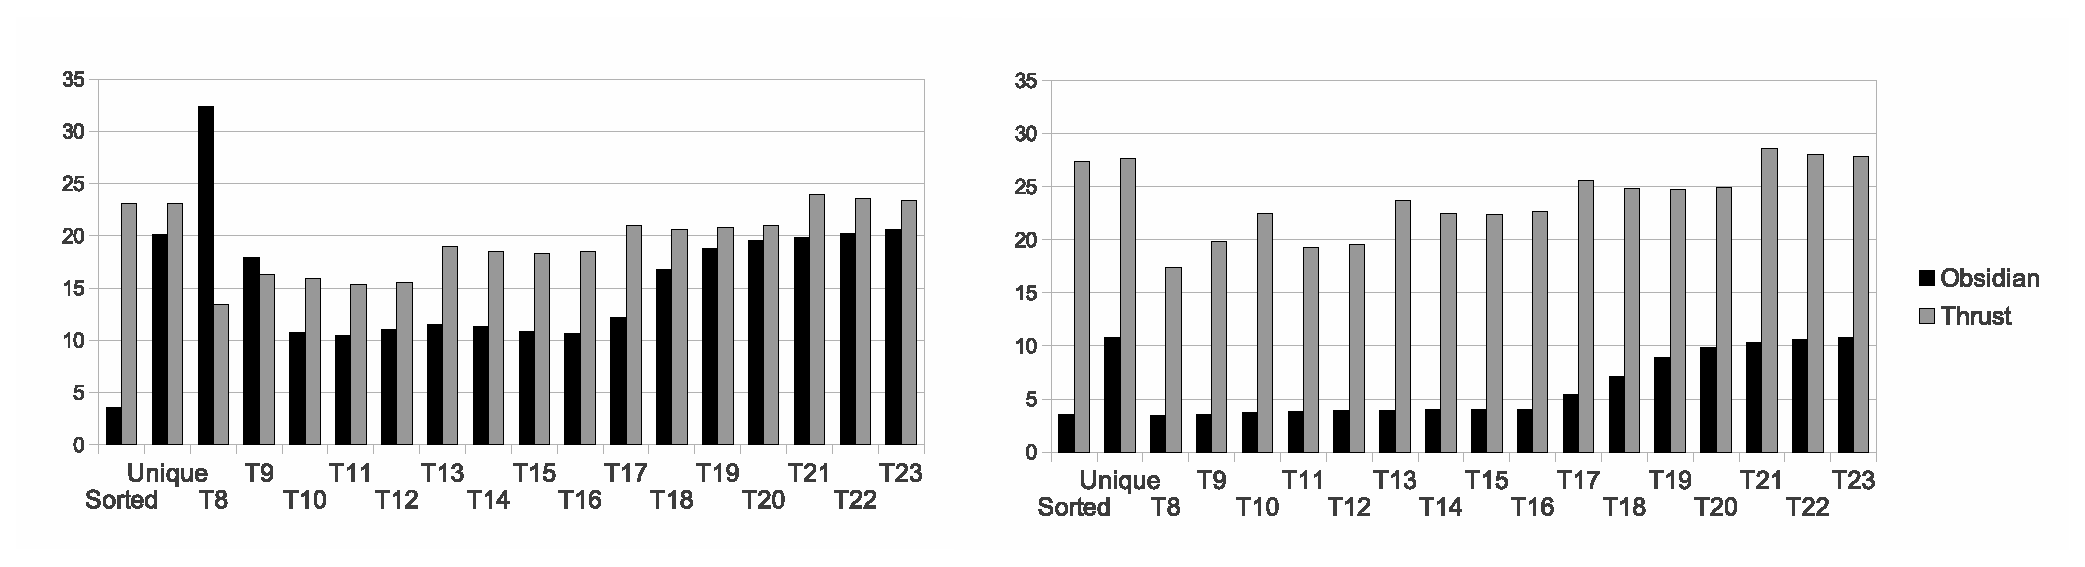
\includegraphics[width=\linewidth]{./img/chart1}
%\caption{Running time and parallel speedup of matrix 
%         multiplication on matrices of different size using ArBB}
%\label{fig:arbbchart}
%\end{figure}


%\begin{figure}
%\includegraphics[width=\linewidth]{./img/arbb1}
%\caption{Execution time for matrix-matrix multiplication using ArBB (C++).
%         Chart shows execution time for various sizes of matrices using 
%         either one two or four cores.}
%\label{fig:arbbchart}
%\end{figure}


%\begin{figure}
%\includegraphics[width=\linewidth]{./img/embarbb1}
%\caption{Execution time for matrix-matrix multiplication using EmbArBB.
%         Chart shows execution time for various sizes of matrices using 
%         either one, two or four cores.}
%\label{fig:embchart}
%\end{figure}

%\begin{figure}
%\includegraphics[width=\linewidth]{./img/repa1}
%\caption{Execution time for matrix-matrix multiplication using Repa.
%         Chart shows execution time for various sizes of matrices using 
%         either one, two, four or eight threads.}
%\label{fig:repachart}
%\end{figure}






%\begin{figure}
%\includegraphics[width=\linewidth]{./img/compare2}
%\caption{CAPTION HERE}
%\label{fig:compare2chart}
%\end{figure}




\FloatBarrier


\section{Related Work} 
\subsection{Data.Array.Accelerate} 
Accelerate~\cite{accelerate} is an embedded language for general purpose, 
flat data parallel computations on GPUs. 

The Accelerate programmer expresses algorithms using collective operations 
over vectors. These collective operations are similar to the 
parallel patterns of ArBB, but are generally higher order. That is, where 
ArBB and EmbArBB have {\tt addReduce}, {\tt mulReduce} and so on, Accelerate
has a single higher-order fold function. This means that the Accelerate library
gets away with a much smaller set of operations, while maintaining a higher 
level of expressivity in the language. 

Accelerate arrays have their dimensionality (shape) encoded in the type 
and this was the inspiration for the similar approach taken in EmbArBB. In 
Accelerate, a one dimensional array of integers has type {\tt Array DIM1 Int}.
However, Accelerate does not limit the dimensionality to one, two or three,
as ArBB does, but rather supports arbitrary dimensionality.

\subsection{Data Parallel Haskell} 
Data Parallel Haskell (DPH) is an extension to GHC for nested data parallelism. 
This is one thing that DPH and ArBB have in common. 
 
In DPH, the programmer can use parallel arrays of type {\tt [:e:]} that look
similar to normal Haskell lists, but give access to data parallel execution.
The similarity to Haskell list processing doesn't end there. The operations 
on these parallel arrays are also reminiscent of Haskell's normal list processing functions.
For example, {\tt mapP}, {\tt unzipP} and {\tt sumP} are parallel versions of 
these well known functions. 

DPH relies on a technique called flattening to transform its nested data parallelism 
into flat data parallelism. 
A recent article about DPH is reference~\cite{DPH}. 
  
 

\subsection{Feldspar} 
Feldspar is a language for Digital Signal Processing (DSP) programming
developed at Chalmers, ELTE University and Ericsson 
(the telecom company)~\cite{FELDSPAR2010}. The functional {\tt while} loop 
of EmbArBB is inspired by the same concept in Feldspar. 

Feldspar is based on a deeply embedded core language and implements 
a vector library as a shallow embedding on top of that. 
This means that there are no vector specific 
constructs in the core abstract syntax. 

%The most recent release of Feldspar uses the {\em Syntactic} library
%for manipulating abstract syntax~\cite{SyntacticICFP12,FELDSYNTACTIC}. 
%We will consider switching to using the Syntactic library in the continued
%implementation of EmbArbb.
%Initial discussions with our colleague Emil Axelsson, the implementor of Syntactic, indicate that
%we should encounter no major difficulties.



\subsection{Nikola} 
Nikola is an embedded language for GPU programming\cite{NIKOLA}, also
in Haskell.  
During the early phases of implementation of EmbArBB, the source code of 
Nikola was often studied for inspiration.

The embedding used in Nikola makes use of an untyped expression 
data structure wrapped up in phantom types, in the style of Pan~\cite{ELLIJFP}.
The EmbArBB embedding works in the same way. 
One of the listed strengths of Nikola is the ability to generate GPU functions 
from Haskell functions, which enables function reuse and the ability to 
amortise the cost of code generation over several launches in an easy 
way. The ability the generate target language function from Haskell functions 
is a present in EmbArBB as well. 

Nikola, like Accelerate, provides a set of higher-order functions with
general {\tt map}, {\tt reduce} and {\tt zipWith} functionality.

\subsection{Repa} 
Repa is a library for regular, shape polymorphic parallel arrays~\cite{REPA}. Repa 
uses a concept of {\tt delayed} arrays to obtain fusion of operations, such as the 
typical map fusion:
\begin{verbatim}
map f . map g  = map (f . g)
\end{verbatim} 
A delayed array 
has a representation that is quite direct to parallelise; it is represented 
as a function from an index-space to an element and the extents of that same 
index-space. Concretely: 

\begin{verbatim} 
data DArray sh e = DArray sh (sh -> e)  
\end{verbatim} 

Parallelising the computation of such an array is done by splitting up the 
index-space over the available parallel resources of the system. Repa does 
not use SIMD (vector) instructions; this is something that ArBB does and 
that EmbArBB gets for free. 

Repa is compared to EmbArBB in the benchmarks in section~\ref{sec:Benchmarks}.

%\subsection{Obsidian}
%Really ? \cite{Obsidian}

\section{Motivation}

We have two main motivations for implementing EmbArBB.

Firstly, we are interested in exploring programming idioms for
data parallel programming in a functional setting. Embedding ArBB gives
a quick route to a platform for such exploration, without too much implementation effort. This is what the ``almost for free'' in the title is intended to refer to.
We wish to explore ways to make use of the fact that we have an array programming library embedded in a sophisticated, strongly typed host language. In our earlier work on the embedded hardware description language Lava, we investigated various approaches to exploiting the host language during netlist synthesis~\cite{LavaMultipliers}, and we have also experimented with the use of search and dynamic programming in generating parallel prefix (or scan) networks~\cite{SheeranJFP}. We intend to apply similar methods to the development of data parallel programs once the EmbArBB implementation is more complete and stable.



%It would be interesting to explore ways of using the host language in more sophisticated ways, rather as we have done for hardware generation in Lava~\cite{LavaMultipliers}.

A second motivation is the desire to teach NESL-style data parallel programming
in a Masters course on parallel functional programming that has recently been
introduced at Chalmers~\cite{TFPIEPFP}. The first instance of the course (in Spring 2012)
covered Blelloch's NESL language, with its
associated cost model~\cite{NESL}, but did not provide any satisfactory way for the students
to experience real, nested data parallel programming. This was due not only to a lack of suitable hardware, but also to deficiencies in the available tools.
We used the Repa library to get flat data parallelism, but then suffered from
the lack of a built-in scan primitive (as many of Blelloch's NESL examples use scan). Perhaps as a result
of needing scan, we did not get good performance.
We have not done enough examples or experiments yet, but it seems to us that EmbArBB
could be used to give students an experience of real parallel programming in a NESL-like
functional language. It remains to be seen whether the limited degree of nesting allowed in ArBB can be offset, at least to some extent, by clever use of the host programming language during generation of the desired abstract syntax tree.


% ------------------------------------------------------------------------------
\section{Future work} \label{sec:fut}

The version of Obsidian described here is at a very experimental stage. 
The quality of the C code generated needs to improve to get performance 
on par with the previous version. The previous version however, was very
limited in what you could express. This older version is described in
\cite{JMT}.
There is a clear opportunity to perform classic compiler optimisations on 
the IC formed by running an Obsidian program. Currently this is not done at all. 

Ways to describe the coordination 
of kernels in code that is still short and sweet are also needed. Some experiments using 
methods similar to Lava's netlist generation have been performed, but the
resulting performance is not yet satisfactory. In CUDA, Kernel coordination 
is in part described in the actual kernel code. Kernels decide which parts 
of the given data to use. As future work we will approach the kernel 
coordination problem at a lower more CUDA-like level. We will, of necessity,
need to develop programming idioms or combinators that express how data is 
placed in the memory hierarchy. The isolation of this as a central question 
is one of the more unexpected and interesting results of the project.
Right now work is focused on developing combinators that are more clever 
in their treatment of {\tt sync}s. This leads to new data structures that 
allow the merging of {\tt sync}s. This new approach seems to make efficient
implementations of combinators such as {\tt two} possible. 



%We also need to experiment with ways of ``moving syncs around'' in our 
%generated code, in order to avoid unnecessary serialisation caused by having 
%too many syncs of small groups of threads.


\subsection{Conclusion} \label{sec:conc}

Obsidian provides a good interface for experimenting with algorithms on GPUs. 
The earlier version described in~\cite{JMT} showed that it is possible to 
generate efficient CUDA code from the kind of high level descriptions we are 
interested in. For the kernel level, the work in progress described in this paper enhances the  expressive power of Obsidian, extending the range of algorithms that can be described, as well as the degree of control exercised by the user. 
Future work will concentrate on improving the performance of the resulting 
applications, as well as on support for the kernel coordination level.

%\bibliographystyle{plain}
%\bibliography{ifl08}

%\end{document}
